\documentclass[11pt,aspectratio=43,ignorenonframetext,t]{beamer}
% Uses fontspec - assumes compiled with LuaLaTeX or similar
% The above \documentclass is for making slides. If making handouts use:
%\documentclass[11pt,a4paper]{article} 
%\usepackage{beamerarticle}
%\setjobnamebeamerversion{main.beamer}

% See https://github.com/CASSON-LAB/uom_beamer_template
% for details on license, further useage information and similar


%%%%%%%%%%%%%%%%%% DOCUMENT SETUP %%%%%%%%%%%%%%%%%%

% \usetheme{AnnArbor}
% \usetheme{Goettingen}
% \usetheme{Madrid}
% \usetheme{Marburg}
% \usetheme{metropolis}
% \usetheme{Darmstadt}
% \usetheme{CambridgeUS}
% \usetheme{Berlin}
% \usetheme{Singapore}

% \usecolortheme{beaver}
% \usecolortheme{spruce}
% \usecolortheme{wolverine}
% \usecolortheme{dolphin}

% Presentation settings
\mode<presentation>{
  \usetheme[framenumber,titleframestart=1]{UoM_alex}
  \usefonttheme{professionalfonts} % using non standard fonts for beamer
  \usefonttheme{serif}             % set font to Arial
  \usepackage{fontspec}
  \setmainfont[Ligatures=TeX]{Arial}
}

% Handout settings
\mode<article>{
  \usepackage{fullpage}                  % use full page
  \usepackage{fontspec}                  % set font to Arial
    \setmainfont[Ligatures=TeX]{Arial}
  \setlength{\parskip}{1.5\baselineskip} % correct beamer line spacings
  \setlength{\parindent}{0cm}
  \usepackage{enumitem}
    \setlist[itemize]{topsep=0pt}
  \definecolor{uomlinkblue}{HTML}{0071BC}
}


% Packages
\usepackage{graphicx}  % for graphics files
  \graphicspath{ {./imgs/} {./screencaps/} }
\usepackage{amsmath}   % assumes amsmath package installed
  \allowdisplaybreaks[1] % allow eqnarrays to break across pages
\usepackage{amssymb}   % assumes amsmath package installed 
\usepackage{unicode-math} % unicode maths for accessibility
\usepackage{pdfcomment} % for alt text for accessibility
\usepackage{rotating}  % allow portrait figures and tables
\usepackage{subfigure} % allow matrices of figures
\usepackage{float}     % allows H option on floats to force here placement
\usepackage{multirow}  % allows merging of rows in tables
\usepackage{tabularx}  % allows fixed width tables
\usepackage{ctable}    % modifies \hline for use in table
\usepackage{bm}        % allow bold fonts in equations
\usepackage{pgf}       % allow graphics manipulation
\usepackage{media9}    % allow interactive flash files to be embedded
  \addmediapath{../media}
\usepackage{etoolbox}
  \makeatletter \preto{\@verbatim}{\topsep=0pt \partopsep=0pt} \makeatother  
\usepackage{colortbl}  %  \arrayrulecolor

% \usepackage{xspace}
% \usepackage{amssymb}
% \usepackage{wasysym}
% \usepackage{mathtools}
% \usepackage{wrapfig}
% \usepackage[TeX,UKenglish]{isodate}

%%  Don't load the natbib package; it will conflict with this
\usepackage[style=authoryear,backend=biber,natbib=true]{biblatex}
\addbibresource{p.bib}

\usepackage{hyperref} % add hyperlinks to document. Settings are for accessiblity
  \hypersetup{
    colorlinks=true,
    linkcolor=uomlinkblue,
    filecolor=uomlinkblue,
    urlcolor=uomlinkblue,
    pdflang={en-GB},
}

% \AtBeginSection{\frame{\sectionpage}}
\AtBeginSection[] % Do nothing for \section*
{
\begin{frame}<beamer>
  \frametitle{Outline}
  \tableofcontents[currentsection]
\end{frame}
}
\setbeamertemplate{footline}[frame number]

%%  https://tex.stackexchange.com/questions/193380/hyperref-pageref-links-point-to-first-page
\newcommand{\hlabel}{\phantomsection\label}

%%  Need to be added to the preamble
%\usepackage{xcolor}

%%  Set colors
\newcommand{\red}[1]{{\color{red}#1}}
\newcommand{\blue}[1]{{\color{blue}#1}}
\newcommand{\green}[1]{{\color{green}#1}}
\newcommand{\magenta}[1]{{\color{magenta}#1}}

\newcommand{\vs}{\vspace{0.5cm}}

%%  Adding labels and referencing labels
\newcommand{\pgref}[1]{page~\pageref{#1}}

\newcommand{\appref}[1]{Appendix~\ref{#1}}
\newcommand{\chapref}[1]{Chapter~\ref{#1}}
\newcommand{\secref}[1]{Section~\ref{#1}}
\newcommand{\subsecref}[1]{Section~\ref{#1}}




%%  Document sections
\newcommand{\newpart}[2]
   {
        \part{#1}
     \label{#2}
   }

\newcommand{\newchapter}[2]
   {
        \chapter{#1}
     \label{#2}
        \setcounter{figure}{0}
   }

\newcommand{\newsection}[2]
   {
        \section{#1}
     \label{#2}
   }

\newcommand{\newsectionstar}[2]
   {
        \section*{#1}
     \label{#2}
   }

\newcommand{\newsubsection}[2]
   {
        \subsection{#1}
     \label{#2}
   }

\newcommand{\newsubsectionstar}[2]
   {
        \subsection*{#1}
     \label{#2}
   }

\newcommand{\newsubsubsection}[2]
   {
        \subsubsection{#1}
     \label{#2}
   }

\newcommand{\newsubsubsectionstar}[2]
   {
        \subsubsection*{#1}
     \label{#2}
   }


%%%%%%%%%%%%%%%%%%%%%%%%%%%%%%%%%%%%%%%%%%%%%%%%%%%
%%  General

%%  Table spacing
\def\D{\hphantom{1}}
\def\C{\hphantom{1,}}
\def\E{\hphantom{\textless}}


%%%%%%%%%%%%%%%%%%%%%%%%%%%%%%%%%%%%%%%%%%%%%%%%%%%
%%  Requires additional packages

%%  Multirow and multicolumn commands
\newcommand{\mc}[2]{\multicolumn{#1}{c|}{#2}}
\newcommand{\mr}[1]{\multirow{2}*{#1}}


%%%%%%%%%%%%%%%%%%%%%%%%%%%%%%%%%%%%%%%%%%%%%%%%%%%
%%  Referencing tables
\newcommand{\tabref}[1]{Table~\ref{#1}}
\newcommand{\subtabref}[2]{Table~\ref{#1}{(#2)}}


%%%%%%%%%%%%%%%%%%%%%%%%%%%%%%%%%%%%%%%%%%%%%%%%%%%
%%  Creating tables

% arg1 = position
% arg2 = column definition string (eg |cc|r|lp{2cm}||)
% arg3 = column headings
% arg4 = body of table
% arg5 = caption
% arg6 = label for the figure
%
\newcommand{\tab}[6]{%
  \begin{table}[#1]
    \centering
      \caption{\label{#6}#5}%
      \begin{tabular}{#2}%
        \hline #3 \hline%
        #4%
        \hline%
      \end{tabular}%
  \end{table}
}

\newcommand{\tabx}[6]{%
  \begin{table}[#1]
    \centering
      \caption{\label{#6}#5}%
      \begin{tabularx}{\linewidth}{#2}%
        \hline #3 \hline%
        #4%
        \hline%
      \end{tabularx}%
  \end{table}
}

\newcommand{\tabstar}[6]{%
  \begin{table*}[#1]
    \centering
      \caption{\label{#6}#5}%
      \begin{tabular}{#2}%
        \hline #3 \hline%
        #4%
        \hline%
      \end{tabular}%
  \end{table*}
}

\newcommand{\tabxstar}[6]{%
  \begin{table*}[#1]
    \centering
      \caption{\label{#6}#5}%
      \begin{tabularx}{\linewidth}{#2}%
        \hline #3 \hline%
        #4%
        \hline%
      \end{tabularx}%
  \end{table*}
}

\newcommand{\sidetab}[6]{%
  \begin{sidewaystable}[#1]
    \centering
      \caption{\label{#6}#5}%
      \begin{tabular}{#2}%
      \hline #3 \hline%
      #4%
      \hline%
      \end{tabular}%
  \end{sidewaystable}
}





%%%%%%%%%%%%%%%%%% FRONT MATTER %%%%%%%%%%%%%%%%%%
\title{Deciding on the ideal software environment}
\subtitle{Personal experiences with Anaconda, Docker, virtual machines, and servers}
\author{Raymond Wan and Patrick Yizhi Cai\\Manchester Institute of Biotechnology\\4 September 2024}
\begin{document}



%%%%%%%%%%%%%%%%%% TITLE SLIDE %%%%%%%%%%%%%%%%%%
\begin{frame}
  \titlepage \hlabel{slide:title}
\end{frame}


%%%%%%%%%%%%%%%%%%%%%%%%%%%%%%%%%%%%%%%%%%%%%%%%%%
\section{Introduction}


%%%%%%%%%%%%%%%%%%%%%%%%%%%%%%%%%%%%%%%%%%%%%%%%%%
\begin{frame}

\frametitle{Introduction}

Prior to project development, two main considerations:
\begin{itemize}
  \item operating systems (i.e., Microsoft Windows, MacOS, or Linux) 
  \item programming language (i.e., Python, C/C++, Java, etc.)
\end{itemize}
\vs

A third but equally important consideration is the {\red{{\emph{environment}}}}.  Some options include:

\begin{itemize}
  \item Anaconda,
  \item Docker,
  \item virtual machines, and
  \item servers
\end{itemize}

i.e., ``inside what'' will the program run -- the focus of this talk

\end{frame}


%%%%%%%%%%%%%%%%%%%%%%%%%%%%%%%%%%%%%%%%%%%%%%%%%%
\begin{frame}

\frametitle{Introduction}

The decision for operating system, programming language, and environment affects all of this:
\begin{itemize}
  \item who should be hired to {\blue{develop}} the project,
  \item who can be brought on to the project to {\green{help}}, and
  \item even how the software will be {\magenta{maintained}}.
\end{itemize}

\end{frame}


%%%%%%%%%%%%%%%%%%%%%%%%%%%%%%%%%%%%%%%%%%%%%%%%%%
\begin{frame}

\frametitle{Outline}

Describe
\begin{enumerate}
  \item briefly, what each of them are,
  \item pros and cons of each, and
  \item what has gone wrong?
\end{enumerate}

\end{frame}


%%%%%%%%%%%%%%%%%%%%%%%%%%%%%%%%%%%%%%%%%%%%%%%%%%
\begin{frame}

\frametitle{Motivation for this talk}

Each promises reproducibility and ease of software maintenance.  Including:
\vs

\begin{itemize}
  \item Reproducing a system from backups on to the same or other system.
  \item Long-term support of a piece of software, possibly by someone who was not the original developer.
\end{itemize}
\vs

But are they all equal?  If they each promise the same thing, how would an RSE choose one over another? \pause

\end{frame}


%%%%%%%%%%%%%%%%%%%%%%%%%%%%%%%%%%%%%%%%%%%%%%%%%%
\begin{frame}

\frametitle{About me}

Obtained a computer science degree in the 1990s and a PhD in computer science in 2004.
\vs

Relevance?  My degrees pre-date all of these:
\begin{itemize}
  \item Anaconda, 
  \item Docker, and
  \item virtual machines
\end{itemize}
\vs

Like many of us, I had to learn them myself.  Regrettably, it means I might not know them very well.

\end{frame}


%%%%%%%%%%%%%%%%%%%%%%%%%%%%%%%%%%%%%%%%%%%%%%%%%%
\section{Overview of each}


%%%%%%%%%%%%%%%%%%%%%%%%%%%%%%%%%%%%%%%%%%%%%%%%%%
\begin{frame}

\frametitle{Servers}

Physical computer (or server):
\begin{itemize}
  \item It can be networked to another computer both inside (intranet) or outside (Internet) a workplace.
  \item Otherwise, no dependencies (or interferences) from other computers.
\end{itemize}

\begin{figure}
  \centering
  
\includegraphics[height=3cm]{imgs/server}
\end{figure}

\end{frame}


%%%%%%%%%%%%%%%%%%%%%%%%%%%%%%%%%%%%%%%%%%%%%%%%%%
\begin{frame}

\frametitle{Servers}

Pros:
\begin{itemize}
  \item Reproducible if you buy a similar computer and install the same software.
  \item Possible to purchase with a research budget since it is a {\blue{fixed}} cost.
\end{itemize}

Cons:
\begin{itemize}
  \item Buying an entire server is a big investment.
  \item Keeping it requires physical space as well as electricity, cooling, physical security, etc.
  \item Someone in-house needs to look after it and act as system administrator.
\end{itemize}

\end{frame}


%%%%%%%%%%%%%%%%%%%%%%%%%%%%%%%%%%%%%%%%%%%%%%%%%%
\begin{frame}

\frametitle{Virtual machines}

\begin{itemize}
  \item Virtualisation\footnote{Dividing of physical computer resources into separate units} at the level of the physical computer.
  \item Host multiple {\green{virtual}} computers on {\red{one}} computer.
  \item On the virtualisation program, you allocate how much memory should be used, disk space, network, etc.
  \item Some {\magenta{programs}}:  Oracle VirtualBox or Microsoft Windows Hyper-V.  Amazon AWS employs the same approach.
\end{itemize}

\begin{figure}
  \centering
  \begin{tabular}{cc}
    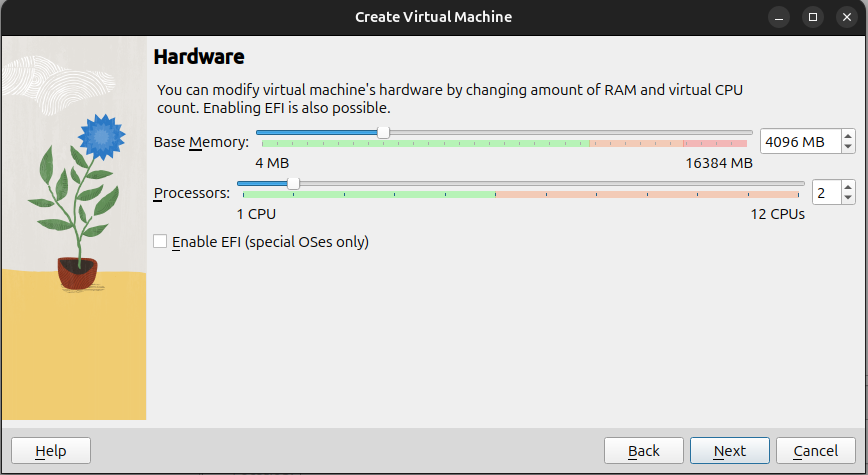
\includegraphics[width=5.25cm]{screencaps/vbox-memory} &
    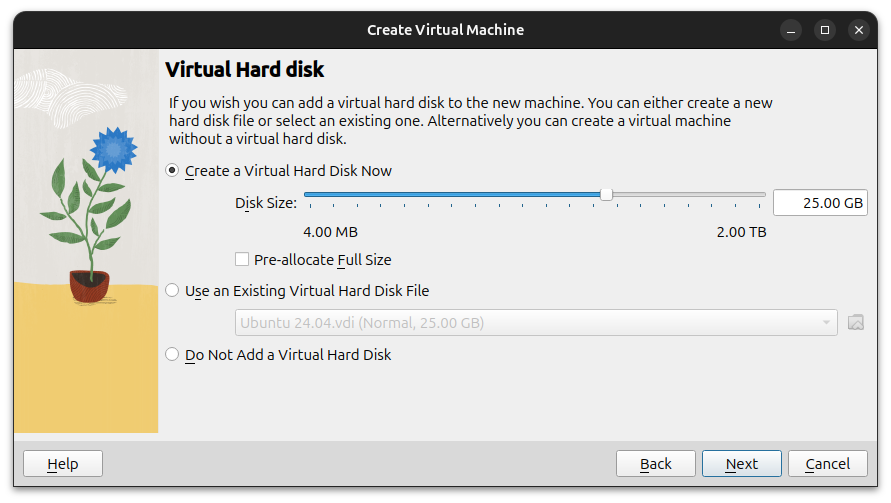
\includegraphics[width=5.25cm]{screencaps/vbox-hdd} \\
  \end{tabular}
\end{figure}

\end{frame}


%%%%%%%%%%%%%%%%%%%%%%%%%%%%%%%%%%%%%%%%%%%%%%%%%%
\begin{frame}

\frametitle{Virtual machines}

\begin{figure}
  \centering
  \includegraphics[width=0.95\textwidth]{screencaps/vbox-partscreen} \\
\end{figure}

\end{frame}


%%%%%%%%%%%%%%%%%%%%%%%%%%%%%%%%%%%%%%%%%%%%%%%%%%
\begin{frame}

\frametitle{Virtual machines}

Pros:
\begin{itemize}
  \item Each VM exists independently of other VMs.
  \item Virtual hard disks can be backed up, copied, and restored on another system.
  \item A snapshot on a live system is possible (with some caveats).
\end{itemize}

Cons:
\begin{itemize}
  \item Common memory, hard disk, and network means that a computationally intensive VM can take up resources from other VMs and the host system.
  \item Some projects require the location of the server and data to be known.  This might rule out Amazon AWS.
\end{itemize}

\end{frame}


%%%%%%%%%%%%%%%%%%%%%%%%%%%%%%%%%%%%%%%%%%%%%%%%%%
\begin{frame}

\frametitle{Docker}

\begin{itemize}
  \item Virtualisation at the level of the operating system, one level above virtual machines.
  \item Unlike before, {\blue{one}} physical computer running {\green{one}} operating system.  On this operating system, Docker Engine is continuously running.
  \item Docker Engine hosts various containers, which are ``self-contained'' software and configuration files.
  \item Multiple Docker containers can be running simultaneously that can communicate with each other.
\end{itemize}

\end{frame}


%%%%%%%%%%%%%%%%%%%%%%%%%%%%%%%%%%%%%%%%%%%%%%%%%%
\begin{frame}

\frametitle{Docker}

Example {\texttt{docker-compose.yml}} for starting up applications based on multiple containers:
\begin{figure}
  \centering
  {\fbox{\begin{tabular}{l}
    version:  '3.0' \\
    services: \\
    {\D\D}helloworld: \\
    {\D\D}{\D\D}container\_name:  hello-world \\
    {\D\D}{\D\D}working\_dir:  /hello \\
    {\D\D}{\D\D}volumes: \\
    {\D\D}{\D\D}{\D\D}- /var/logs/helloworld:/myapp/logs \\
    ...\\
  \end{tabular}
  }}
\end{figure}

\begin{itemize}
  \item {\texttt{/hello}} and {\texttt{/var/logs/helloworld}} are directories on the {\blue{host}} computer
  \item {\texttt{/myapps/logs}} is from the point of view of the application
\end{itemize}

\end{frame}


%%%%%%%%%%%%%%%%%%%%%%%%%%%%%%%%%%%%%%%%%%%%%%%%%%
\begin{frame}

\frametitle{Docker}

Pros:
\begin{itemize}
  \item Good for programs that start up, run, and end (i.e., for data processing/analysis, etc.).
  \item Some developers use it to write web applications.
\end{itemize}

Cons:
\begin{itemize}
  \item With less separation from the host compared to virtual machines, diagnosing problems (i.e., why does it work on this computer but not that one) can be frustrating.
  \item {\magenta{Personally}}, a steeper learning curve than the other options.
\end{itemize}

\end{frame}


%%%%%%%%%%%%%%%%%%%%%%%%%%%%%%%%%%%%%%%%%%%%%%%%%%
\begin{frame}

\frametitle{Anaconda}

\begin{itemize}
  \item Able to manage separate instances of Python and R, as well as other open source programs.
  \item Software packages are grouped together into Anaconda {\green{environments}}.
  \item Same program at different versions can be installed in multiple environments by the same user.
\end{itemize}
\vs

Example setup on Ubuntu host:
\begin{figure}
  \centering
  \begin{tabular}{ll}
    \hline
    \multicolumn{1}{c}{Command} & \multicolumn{1}{c}{What it does} \\
    \hline
    {\texttt{sudo apt-get install bwa}} & Install {\texttt{bwa}} on host \\
    \arrayrulecolor{red}\hline
    {\texttt{conda create --name rsecon24}} & Create an environment \\
    {\texttt{conda activate rsecon24}} & Activate environment \\
    {\texttt{conda install bwa}}       & Install {\texttt{bwa}} in environment \\
    \arrayrulecolor{black}\hline
  \end{tabular}
\end{figure}

\end{frame}


%%%%%%%%%%%%%%%%%%%%%%%%%%%%%%%%%%%%%%%%%%%%%%%%%%
\begin{frame}

\frametitle{Anaconda}

\begin{figure}
  \centering
  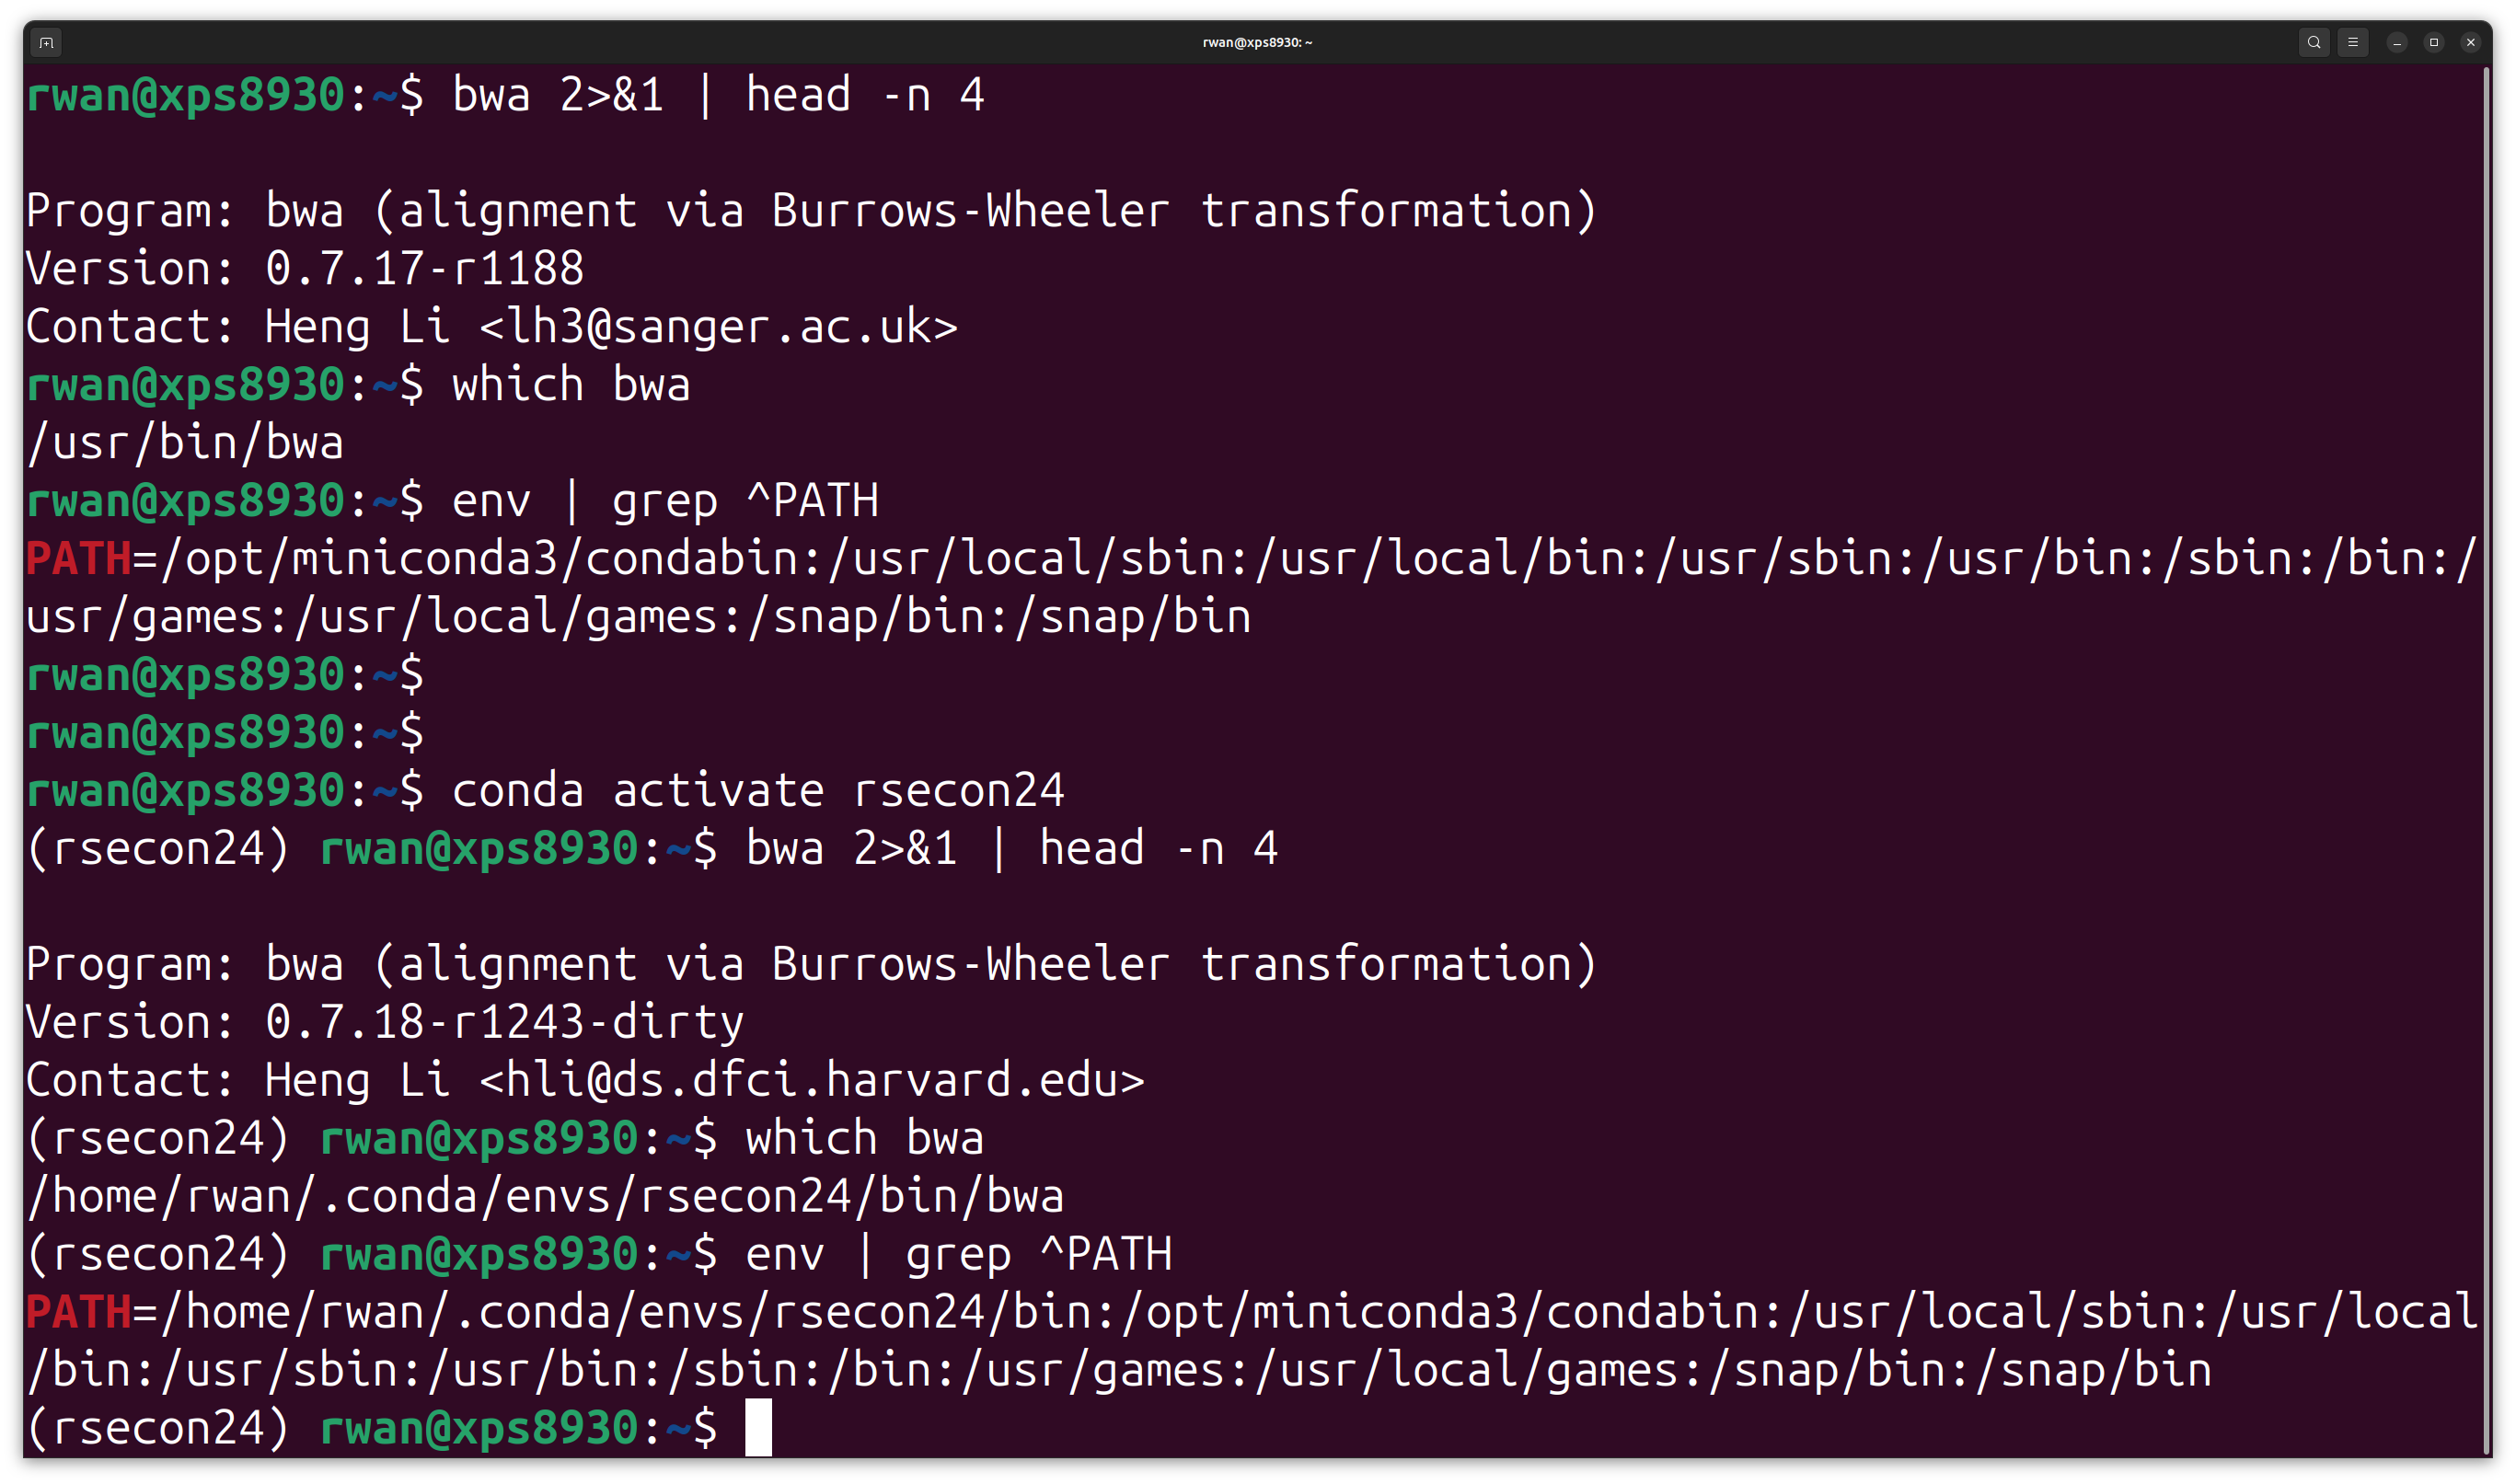
\includegraphics[width=\textwidth]{screencaps/anaconda}
\end{figure}

\end{frame}


%%%%%%%%%%%%%%%%%%%%%%%%%%%%%%%%%%%%%%%%%%%%%%%%%%
\begin{frame}

\frametitle{Anaconda}

\begin{figure}
  \centering
  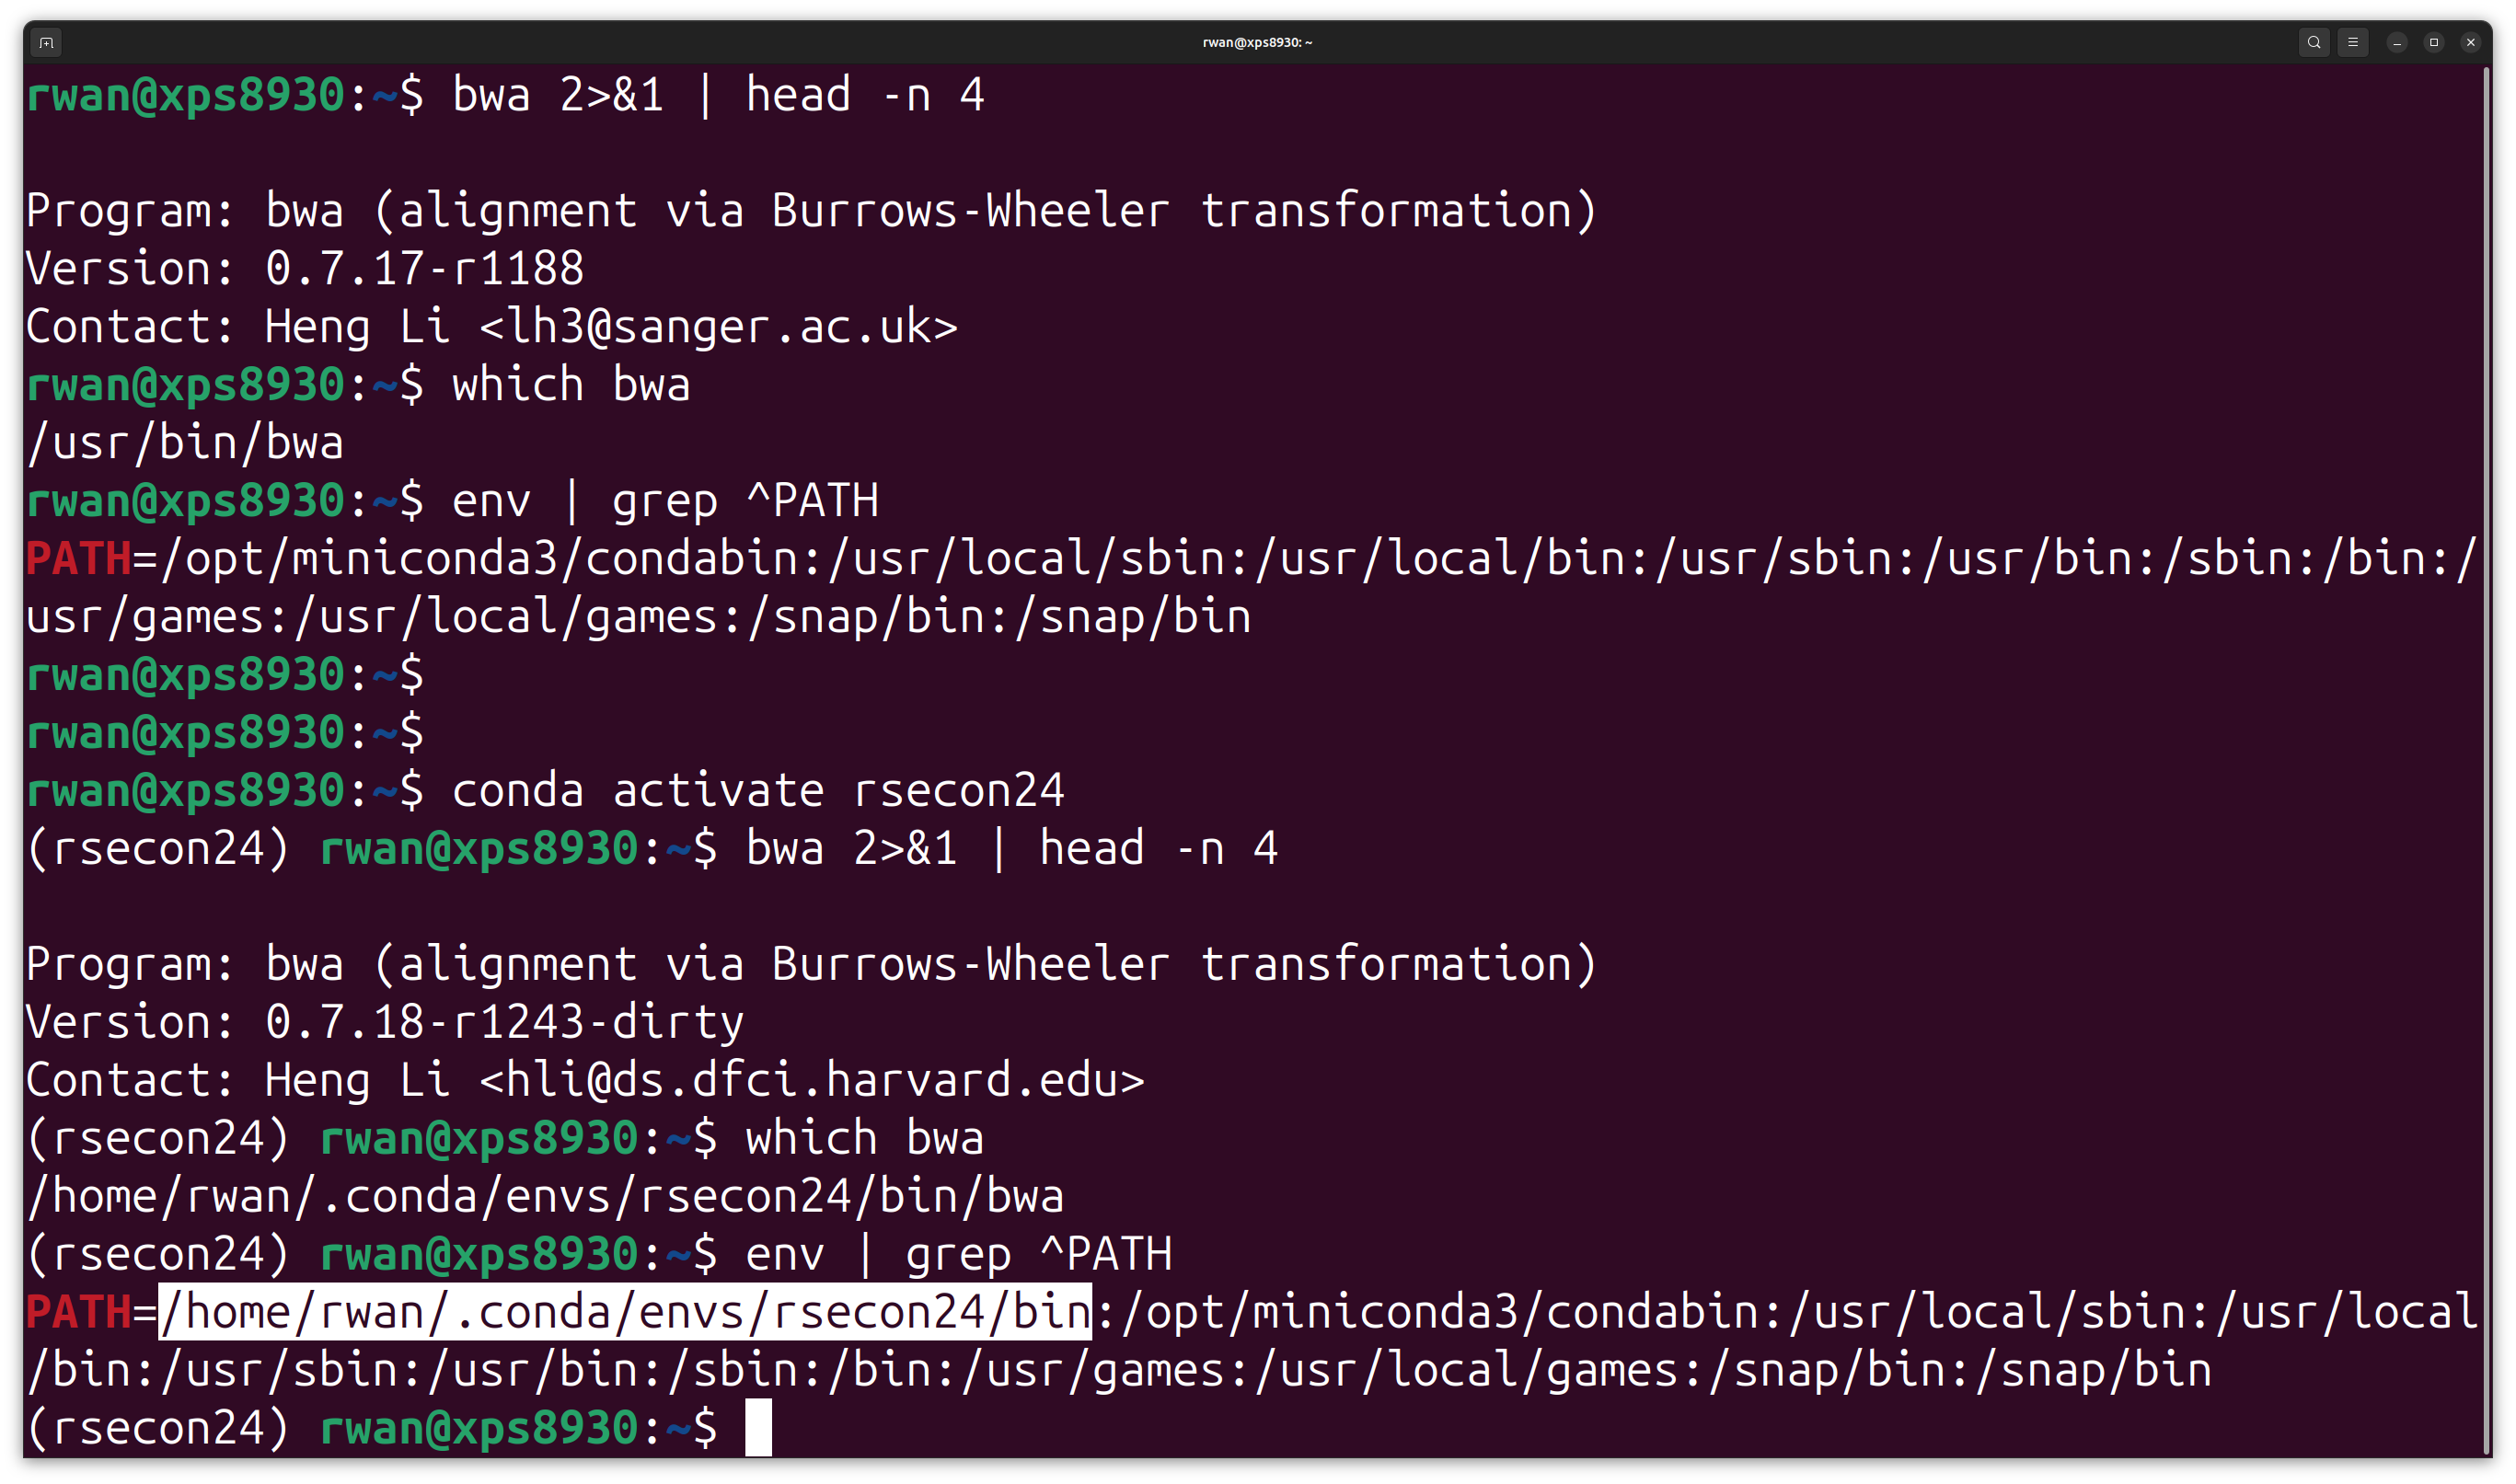
\includegraphics[width=\textwidth]{screencaps/anaconda-highlight}
\end{figure}

\end{frame}


%%%%%%%%%%%%%%%%%%%%%%%%%%%%%%%%%%%%%%%%%%%%%%%%%%
\begin{frame}

\frametitle{Anaconda}

Pros:
\begin{itemize}
  \item Relatively very little setup.  Anaconda can be installed by a user or the system administrator.  Then, the user can create and delete their own Anaconda environments.
  \item Neither Oracle VirtualBox nor a Docker Engine-like system is running.
  \item Conceptually easier to understand; it's ``just'' updating the user's {\texttt{PATH}}.
  \item Ideal for data analysis; not useful for writing a web application.
\end{itemize}

Cons:
\begin{itemize}
  \item No separation between environments and between environments and the host system.
\end{itemize}

\end{frame}


%%%%%%%%%%%%%%%%%%%%%%%%%%%%%%%%%%%%%%%%%%%%%%%%%%
\begin{frame}

\frametitle{Summary}

\begin{figure}
  \centering
  
\includegraphics[width=\textwidth]{inkscape/summary}
\end{figure}

We all want less complexity:
\begin{itemize}
  \item Lower financial costs
  \item Anaconda environments can be created and maintained without system administrator access
\end{itemize}
\vs

More isolation makes it easier to reproduce an environment and/or troubleshoot.

\end{frame}


%%%%%%%%%%%%%%%%%%%%%%%%%%%%%%%%%%%%%%%%%%%%%%%%%%
\section{What has gone wrong?}


%%%%%%%%%%%%%%%%%%%%%%%%%%%%%%%%%%%%%%%%%%%%%%%%%%
\begin{frame}

\frametitle{Layered organisation}

\begin{figure}
  \centering
  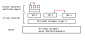
\includegraphics[width=\textwidth]{inkscape/layers}
\end{figure}

With communication (in {\red{red}}) between Docker containers and virtual machines.
\vs

At first glance, it should help with reproducibility...

\end{frame}


%%%%%%%%%%%%%%%%%%%%%%%%%%%%%%%%%%%%%%%%%%%%%%%%%%
\begin{frame}

\frametitle{Layered organisation}

\hypertarget{slide:layered}{In practice}, when something goes wrong (i.e., network connection failed or one Docker container not communicating with another), finding the cause is difficult...
\vs

Occasionally, the server's operating system or a virtual machine's OS should be upgraded.  If it fails, then anything that depends on it will be affected.  Thus, many systems can fail at the {\green{same time}}.
\vs

Also, see {\hyperlink{slide:eol}{this}}.

\end{frame}



%%%%%%%%%%%%%%%%%%%%%%%%%%%%%%%%%%%%%%%%%%%%%%%%%%
\begin{frame}

\frametitle{Dependencies}

\hypertarget{slide:dependencies}{As} part of ``software reuse'', most software depend on modules, libraries, packages, etc. created by others.
\vs

If one of those dependencies is ever removed or made redundant, then restoring the system from backups would be difficult.  This is less likely when the system is first completed; and more likely during the software's {\magenta{maintenance period}}.
\vs

My own experience is that this is less likely at the operating system level (i.e., Debian/Ubuntu packages) and more likely when:
\begin{itemize}
  \item Re-creating Docker containers
  \item Re-creating Anaconda environments
\end{itemize}

See {\hyperlink{slide:removedpkgs}{this}} for some personal examples.

\end{frame}


%%%%%%%%%%%%%%%%%%%%%%%%%%%%%%%%%%%%%%%%%%%%%%%%%%
\begin{frame}

\frametitle{Rebooting systems}

Message on my phone:
\begin{figure}
  \centering
  {\fbox{
\includegraphics[width=5cm]{imgs/android-restart}}}
\end{figure}
\vs

Restarting computers and software as a solution used to be a punch-line to a joke.  Now, it is actually recommended...
\vs

Due to the two previous reasons, we avoided restarting the entire system.  Ultimately, we were delaying the inevitable.

\end{frame}


%%%%%%%%%%%%%%%%%%%%%%%%%%%%%%%%%%%%%%%%%%%%%%%%%%
\section{Summary}


%%%%%%%%%%%%%%%%%%%%%%%%%%%%%%%%%%%%%%%%%%%%%%%%%%
\begin{frame}

\frametitle{Which to choose?}

\begin{itemize}
  \item Each has its pros and cons.
  \item If one option has issues, then it would have disappeared by now.
  \item Best is to know when to use one over another, instead of using one for everything.
\end{itemize}

\end{frame}


%%%%%%%%%%%%%%%%%%%%%%%%%%%%%%%%%%%%%%%%%%%%%%%%%%
\begin{frame}

\frametitle{Which to choose?}

\begin{itemize}
  \item Server -- If server or data location is an issue {\blue{and}} if physical space and someone to look after it is available.
  \item Virtual machine -- Alternative to buying a new server; but the host computer needs to be {\green{powerful}} enough to support multiple running operating systems.
  \item Docker -- Slightly steeper learning curve than the other options, but worth the time invested as an {\magenta{intermediate}} option between virtual machines and Anaconda.
  \item Anaconda -- Allow users without system administrator's access to create their own environments and install their own software.  They can install {\red{multiple}} versions of Python or R (i.e., 4.4.1, 3.6.1, ...) in separate environments to accommodate their code.
\end{itemize}

\end{frame}


%%%%%%%%%%%%%%%%%%%%%%%%%%%%%%%%%%%%%%%%%%%%%%%%%%
\begin{frame}

\frametitle{Other advice}

Good to periodically {\green{re-create}} Docker containers and Anaconda environments from scratch on another system.  Just to check that its external dependencies are all fine.  Doing this when we're ``free'' means we can confront these problems on our own terms.
\vs

Lastly, I am not yet convinced if layers of environments is a good approach.

\end{frame}


%%%%%%%%%%%%%%%%%%%%%%%%%%%%%%%%%%%%%%%%%%%%%%%%%%
\begin{frame}

\frametitle{Conclusion}

None of these environments is a good substitute for good {\magenta{documentation}}.
\vs

That is, step-by-step instructions that explains how everything fits together.

\end{frame}


%%%%%%%%%%%%%%%%%%%%%%%%%%%%%%%%%%%%%%%%%%%%%%%%%%
\begin{frame}

\frametitle{Acknowledgements}

We thank
\begin{itemize}
  \item colleagues in my current and all previous workplaces for their patience while I learned all this,
  \item reviewers for the helpful suggestions, and
  \item the organising committee for the opportunity to present our experiences.
\end{itemize}

\end{frame}


%%%%%%%%%%%%%%%%%%%%%%%%%%%%%%%%%%%%%%%%%%%%%%%%%%
\begin{frame}

\frametitle{Contact details}

\begin{table}
  \begin{tabular}{c}
  Raymond Wan and Patrick Yizhi Cai\\
  {\texttt{\{raymond.wan,yizhi.cai\}@manchester.ac.uk}}\\
  Manchester Institute of Biotechnology, University of Manchester\\
  \end{tabular}
\end{table}
\vs

\LaTeX\ slides:  \href{https://github.com/rwanwork/Conf_RSECon_2024}{https://github.com/rwanwork/Conf\_RSECon\_2024}
\vs

Homepage of the lab:  \href{https://www.cailab.org/}{https://www.cailab.org/}
\vs

\begin{center}
  {\red{Thank you!}}
\end{center}

\end{frame}


%%%%%%%%%%%%%%%%%%%%%%%%%%%%%%%%%%%%%%%%%%%%%%%%%%
\begin{frame}

\frametitle{License}

These slides and its \LaTeX\ source are released under the Creative Commons Attribution-NonCommercial-ShareAlike 4.0 International License.
\vs

\begin{figure}
  \centering
  
\includegraphics[width=5cm]{imgs/by-nc-sa}
\end{figure}

See \href{https://creativecommons.org/licenses/by-nc-sa/4.0/}{https://creativecommons.org/licenses/by-nc-sa/4.0/} for further details.

\end{frame}


%%%%%%%%%%%%%%%%%%%%%%%%%%%%%%%%%%%%%%%%%%%%%%%%%%
\begin{frame}

\frametitle{Additional credits}

\begin{itemize}
  \item \LaTeX\ template from:  \href{https://www.overleaf.com/latex/templates/university-of-manchester-presentation-beamer-template/rwcrzjmzcdyn}{https://www.overleaf.com/latex/templates/university-of-manchester-presentation-beamer-template/rwcrzjmzcdyn}.
  \item Server clip art from \href{https://clipart-library.com/}{Clipart Library}.
  \item Other figures made using \href{https://inkscape.org/}{Inkscape} version 1.2.2
\end{itemize}

\end{frame}


%%%%%%%%%%%%%%%%%%%%%%%%%%%%%%%%%%%%%%%%%%%%%%%%%%
\begin{frame}

\frametitle{End of Life}

\hypertarget{slide:eol}{End of Life} of software occurs when it is no longer supported by the original developer.  No more support is given and no security updates are made available.
\vs

In our case, \href{https://en.wikipedia.org/wiki/Windows\_Server\_2012\_R2}{support} for Microsoft Windows Server 2012 R2 Datacentre would have ended on 10 October 2023.  So, a major update had to occur or else we would lose security updates and, likewise, the ability to connect to our organisation's network.
\vspace{3cm}

{\hfill}{\hyperlink{slide:layered}{Back}}

\end{frame}


%%%%%%%%%%%%%%%%%%%%%%%%%%%%%%%%%%%%%%%%%%%%%%%%%%
\begin{frame}

\frametitle{Removed packages}

\hypertarget{slide:removedpkgs}{When} a module, a library, or a package is no longer available, substituting it for a newer version might not be possible if the newer version is {\red{not}} backward compatible.
\vs

Also, another module that depends on it in turn might also have to be upgraded, causing a {\blue{ripple}} effect.
\vs

In the past, solving such problems has taken me hours or days.

\end{frame}


%%%%%%%%%%%%%%%%%%%%%%%%%%%%%%%%%%%%%%%%%%%%%%%%%%
\begin{frame}

\frametitle{Removed packages}

In our case, a web application developed using Ruby on Rails had one of its dependencies (mimemagic) removed from all repositories due to a licensing issue.  This occurred after our software had been developed and during its post-development maintenance period.
\vs

See this \href{https://dev.to/cseeman/what-s-up-with-mimemagic-breaking-everything-he1}{page} for an explanation.
\vspace{3cm}

{\hfill}{\hyperlink{slide:dependencies}{Back}}

\end{frame}


%%%%%%%%%%%%%%%%%% END MATTER %%%%%%%%%%%%%%%%%%
\end{document}
